\chapter{Понятие об изохронной и полной вариациях функции. Действие по
Гамильтону. Принцип наименьшего действия Гамильтона-Остроградского.}

Рассмотрим функцию времени \( t \) и некоторого параметра \( \alpha \)
\( q=q(\alpha, t) \). Величина 
\[
    \delta q= \pder{q}{\alpha} d\alpha
\]
называется \textit{изохронной вариацией} (совпадает с виртуальным перемещением),
а величина
\[
    \Delta q= \delta q + d q = \pder{q}{\alpha} d\alpha + \pder{q}{t}\,dt
\]
называется \textit{полной вариацией}.


\sidefig(9cm)
{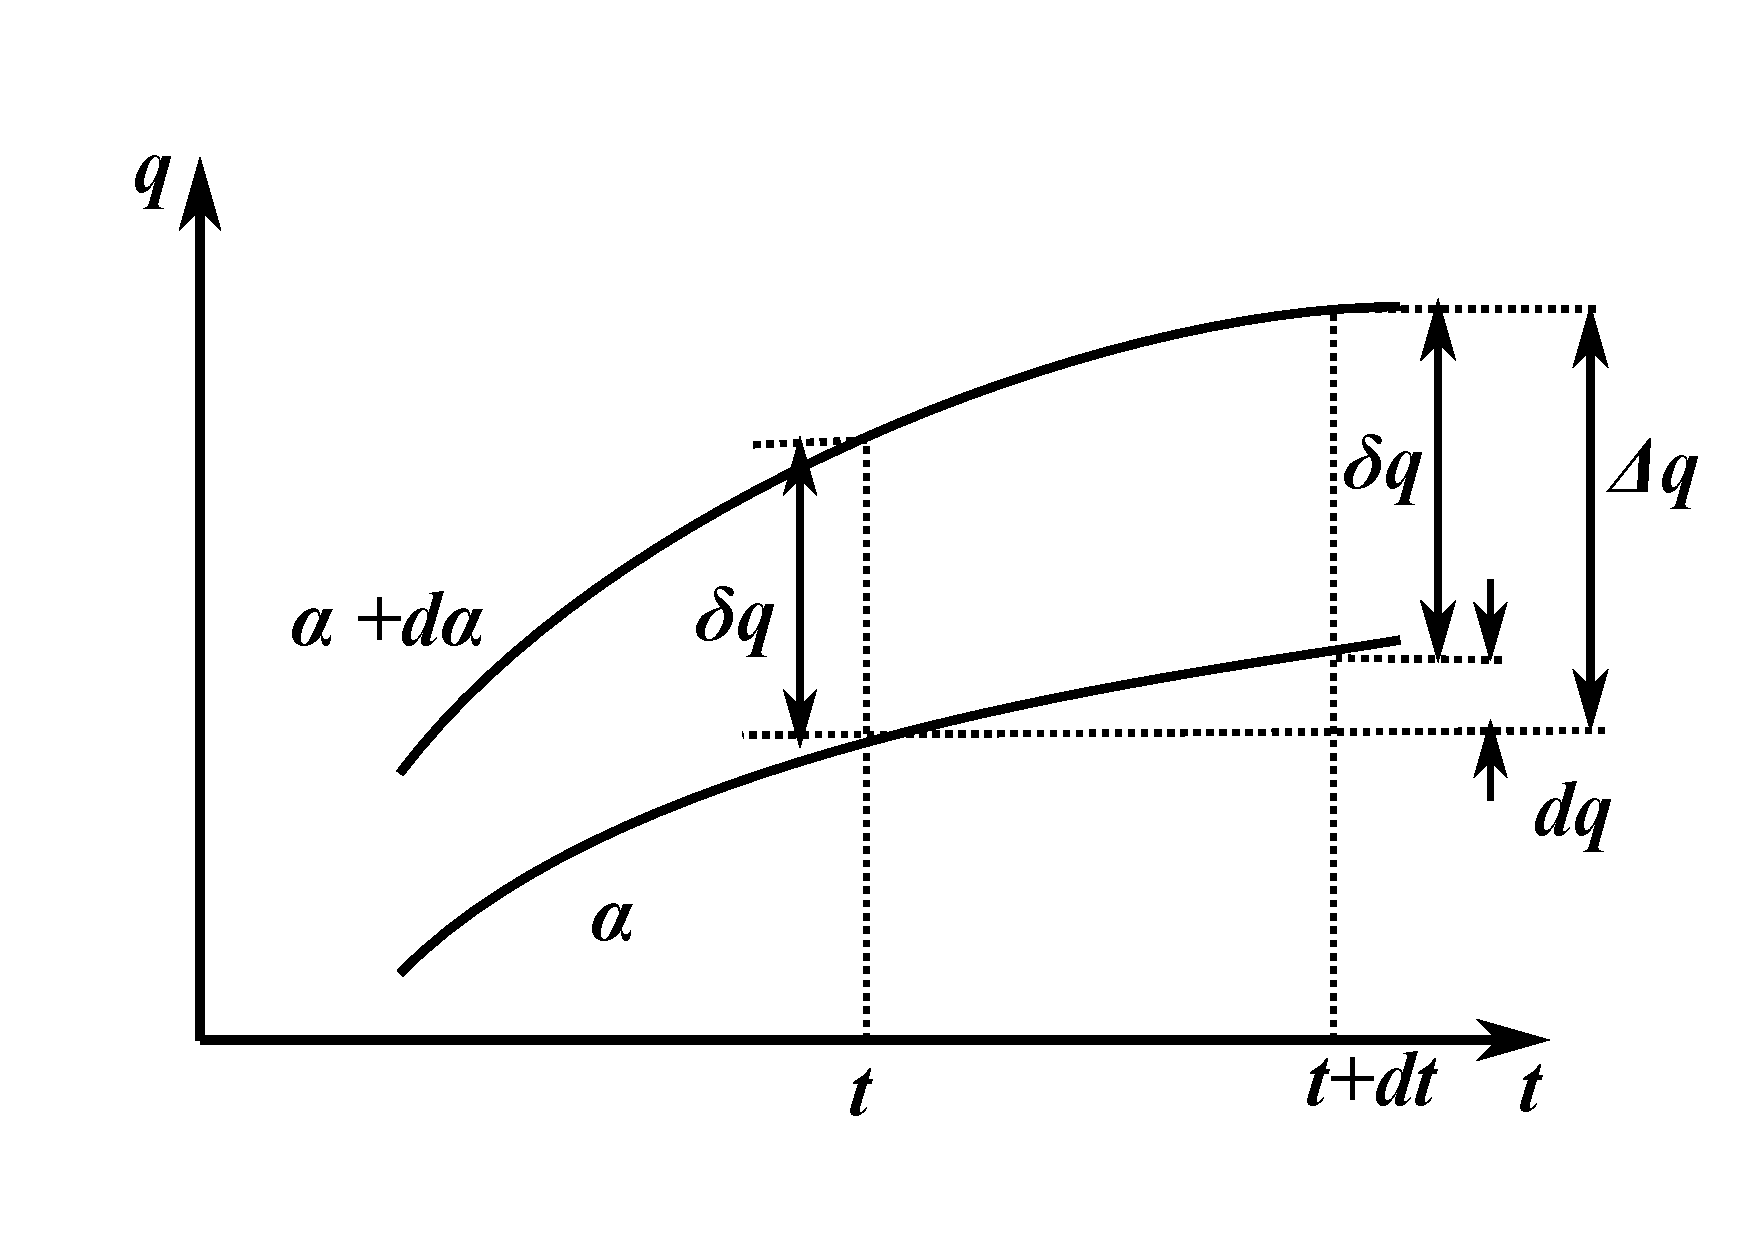
\includegraphics[width=\textwidth]{10}}
{Всё это демонстрируется рисунком справа.

\textit{Действием по Гамильтону} называется интеграл от функции Лагранжа:
\[
        S = \int\limits_{t_0}^{t_1} L\,dt.
\]
}   
\textbf{Принцип наименьшего действия Гамильтона-Остроградского:} \emph{действие
по Гамильтону в истинном движении достигает стационарного значения по сравнению
со значениями на всех близких движениях. Только в истинном движении изохронная
вариация действия по Гамильтону равна \( 0 \):}
\[
    \delta S = 0.
\]

Ограничения на принцип:
\begin{itemize}
\item механическая система должна быть голономна;
\item все сравниваемые движения начинаются в один и тот же момент времени и
    заканчиваются в один и тот же момент времени;
\item изохронные вариации в начальный и конечный момент нулевые.
\end{itemize}

Покажем эквивалентность принципа наименьшего действия и уравнений Лагранжа:
\[
    \delta S =
    \pder{S}{\alpha}\delta\alpha =
    \int\limits_{t_0}^{t_1} \pder{L}{\alpha} d\alpha\,dt =
    \int\limits_{t_0}^{t_1} \delta{L}\,dt.
\]
Но 
\[
    \delta{L} =
    \delta{L}(q_1,\dots,q_s, \dot{q}_1, \dots,  \dot{q}_s, t) =
    \sum\limits_{i=1}^s 
    \pder{L}{q_i}\delta q_i
    +
    \sum\limits_{i=1}^s 
    \pder{L}{\dot{q}_i}\delta\dot{q}_i.
\]
Тогда 
\begin{gather*}
    \int\limits_{t_0}^{t_1} \delta{L}\,dt=
    \sum\limits_{i=1}^s
    \int\limits_{t_0}^{t_1}
    \left(
    \pder{L}{q_i} \delta q_i+
    \pder{L}{\dot{q}_i} \delta  \dot{q}_i
    \right)dt = \\ =
    \sum\limits_{i=1}^s
    \left[
    \int\limits_{t_0}^{t_1}
    \left(
    \pder{L}{q_i} -
    \der{}{t}\pder{L}{\dot{q}_i} 
    \right)\delta  {q}_i\,dt
    +
    \left.  
    \pder{L}{\dot{q}_i} \delta  {q}_i  
    \right|_{t_1}^{t_2}
    \right] =
    \sum\limits_{i=1}^s
    \int\limits_{t_0}^{t_1}
    \left(
    \pder{L}{q_i} -
    \der{}{t}\pder{L}{\dot{q}_i} 
    \right)\delta  {q}_i\,dt.
\end{gather*}

А так как \( \delta q_i \) - независимы
\[
    \der{}{t}\pder{L}{\dot{q}_i} - \pder{L}{q_i} = 0 \quad (i=1,2,\dots,s),
\]  
т. е. мы получили уравнения Лагранжа. Все выкладки обратимы, а значит
эквивалентность доказана. 

\newpage
